%\documentclass[10pt,sigplan,screen,review,anonymous]{acmart}
\documentclass[10pt,sigplan,screen,anonymous]{acmart}
%\documentclass[10pt,manuscript]{acmart}

\setcopyright{none}
\settopmatter{printacmref=false}
\renewcommand\footnotetextcopyrightpermission[1]{}

%\acmConference[SBLP 2025]{29th Brazilian Symposium on Programming Languages}{September, 22--26, 2025}{Recife, PE}

%\usepackage{babel}
%\widowpenalty=10000
%\clubpenalty=10000
\tolerance=500 % acceptable white space in a line, using hyphens
\pretolerance=5100 % acceptable white space in a line, without hyphens
\emergencystretch=1pt %extra space per line
\righthyphenmin=3
\lefthyphenmin=2

% robcmp syntax
\usepackage{roblang}

\newcommand{\blindreview}[1]{{\color{teal}{<omitted for blind review>}}}
%\newcommand{\blindreview}[1]{#1}



\begin{document}

%\title{Hardware Abstraction through Compile-Time Dependency Injection in Embedded Systems}
%\title{Compile-Time Dependency Injection for Hardware Abstraction in Embedded Systems}
%\title{Compiler-Assisted Dependency Injection for Hardware Abstraction in Embedded Systems}
%\title{Compiler-Driven Dependency Injection for Hardware Abstraction in Embedded Software}
\title{A Compiler-Driven Approach for Static Dependency Injection in Embedded Software}


\begin{abstract}
Developing embedded software is challenging due to the need to strike a balance between writing loosely coupled and maintainable code while coping with the microcontroller's limitations in memory, storage, and processing power. While object-oriented programming can lead to improved abstractions and cohesive, easier-to-maintain software, traditional low-level implementation of polymorphism often introduces runtime overhead that hinders its adoption. This paper proposes a compiler-driven dependency injection (DI) technique that enables the compiler to resolve dependencies and replace bound interfaces with concrete implementations in the AST tree to reduce the burden of virtual dispatch in embedded software. We compared five implementations of a breakout game written with object-oriented language features, C++20 concepts, and our proposed method. Results show that the language features allow clear interface definitions and centralized binding configurations, enhancing maintainability and portability. Furthermore, our compiler-driven approach enables optimizations beyond interface boundaries, improving code inlining, constant propagation, interprocedural optimization, and dead code elimination, producing 41.9\% smaller and up to 73.3\% faster firmware than equivalent versions with compile-time injection.
\end{abstract}

\keywords{Compiler-driven dependency injection; Embedded software; Hardware Abstraction; Optimization}

\maketitle

\section{Introduction}

Embedded systems pose unique challenges to software design due to the inherent resource constraints of microcontrollers, which include limited memory, storage, and processing power, as well as application-specific constraints such as security, energy consumption, weight, and cost limitations \cite{buttazzo2006}. Frequently, supporting multiple hardware architectures is also a firmware requirement or becomes a necessity when designing new product versions with upgraded hardware. These constraints require efficient software, typically tightly coupled with hardware using low-level features of programming languages to configure and manage the microcontroller units (MCUs) \cite{varoumas2023}.

While these methods of coping with hardware heterogeneity and product requirements are functional and widely used, they often lead to reduced software cohesion and tightly coupled code to hardware architecture, obscuring its structure and making it harder to maintain and debug. That is particularly true when targeting multiple platforms, as the platform-specific details increase, resulting in maintenance challenges, higher complexity, and decreased portability \cite{pappas2024semantic,ernst2002empirical,cppdesign}.

In turn, principles from object-oriented programming (OOP) such as encapsulation, inheritance, and polymorphism can improve software cohesion and reduce coupling by promoting a clear separation between hardware-specific code and application logic through standardized interfaces. However, the standard low-level implementation of these principles provokes additional code size and performance overhead due to dynamic dispatch mechanisms, such as virtual function tables (vtables) and supporting structures \cite{bauer2021novt}. To address these inefficiencies, generic programming and metaprogramming are options available in languages (such as C++ and Rust), which provide flexible and type-safe abstractions, enabling static polymorphism and not incurring runtime overhead \cite{juhasz2023modern}. Nevertheless, their use increases the complexity of code maintenance and sometimes introduces challenges related to code size (code or template bloat) due to the monomorphization technique employed during the compilation \cite{rust2022} -- a significant constraint in embedded software development.


Dependency Injection (DI) \cite{seemann2019dependency}, often overlooked in embedded system software, is a technique commonly used in object-oriented programming to separate the concern of how dependencies are provided to a component from the component's core logic. The key advantages of DI are enhanced modularity, testability, and flexibility, which result in easier maintenance in general and can enable portability for hardware or peripheral changes independently of the core application logic in embedded software. However, as DI frameworks are built on top of OOP, they share the same disadvantages discussed for dynamic dispatch. Additionally, the need for runtime resolution of dependencies introduces performance overhead due to the use of Run-Time Type Information (RTTI or reflection). Furthermore, DI containers can complicate dependency tracking, making it more challenging to debug the firmware due to reduced predictability, especially when managing low-level hardware-software interactions.

However, recent advances in DI frameworks sacrifice flexibility for runtime performance by resolving dependencies at compile time, thus eliminating the need for reflection and reducing dynamic dispatch (e.g., the Dagger 2 framework \cite{dagger2} for Java and Boost-ext.di for C++ \cite{boostdi2018}). Despite that, they still are external libraries outside the compiler's core, leaving the compiler unaware of the concrete types associated with abstract interfaces. Additionally, these frameworks typically rely on complex template metaprogramming constructs (see Section \ref{sec:breakout}), which can increase the cognitive burden for developers. 

In this paper, we further expand compile-time dependency injection, evaluating a novel compiler-driven approach for embedded software. In addition to generating code that instantiates and injects dependencies at compile time, we also make the compiler frontend aware of the bindings and capable of replacing bound interfaces entirely with their concrete implementations in the abstract syntax tree (AST). This deeper integration enables the compiler's intermediate code generation to optimize beyond opaque interface boundaries, significantly increasing the number of static calls and improving the efficiency of optimization passes such as inlining \cite{damasio2021}, constant propagation, interprocedural optimization (IPO), and dead code elimination (DCE) \cite{cooper2021compiler}, resulting in smaller binaries and faster execution. We argue that this approach also simplifies hardware abstraction, improves early error detection, and enhances maintainability compared to object-oriented programming using vtables and generic programming/metaprogramming using C++20 concepts.


The remainder of this paper is organized as follows. In Section~\ref{sec:di}, we discuss runtime and compile-time dependency injection as well as their limitations regarding embedded software constraints. In Section~\ref{sec:ledblink}, we introduce the syntax of the language features that support our approach through an easy-to-follow example. Section~\ref{sec:design} describes the compiler-driven DI and discusses our implementation choices. Section~\ref{sec:breakout} begins the evaluation, comparing five versions of a breakout game concerning its software quality attributes, followed by a performance evaluation in Section~\ref{sec:performance}. Finally, we present our conclusion and propose future work in Section~\ref{sec:conclusion}.


\section{Dependency Injection} \label{sec:di}
 
Suppose that in the source code of a firmware, we have a class representing an MCU hardware with inner classes abstracting each of its digital ports. Each of these subclasses implements a {\tt digitalport} interface that has methods to set the port direction (input/output) and to get or set its value. A digital port then becomes a component that other classes for hardware peripherals can depend on. For example, a class (or driver) for an SPI display can depend on ports for tasks such as selecting, resetting, and sending data or commands to draw pixels in the display panel. The specific ports used to interconnect these two hardware components vary significantly across different hardware designs or MCUs. The process of mapping, in software, the hardware connections of the circuit board becomes increasingly challenging as the firmware increases support for products from distinct vendors (3D printer firmware, for example \cite{marlinfwm2025}).
 
Dependency injection (DI) \cite{seemann2019dependency} is a design pattern built on top of OOP that implements the principle of inversion of control. Given a set of binding rules, a DI framework implements an external entity responsible for providing the dependencies required by a software component. In the example above, a set of rules in the application configuration determines what digital ports to bind to the SPI display without hard-coding it in the display class. This way, the display class becomes modular and can even be tested with mocked ports when unit testing the software. Thus, by decoupling component configuration from implementation logic, DI promotes modularity, testability, and reuse \cite{seemann2019dependency,garousi2019}.

Most popular DI frameworks target general-purpose environments with dynamic runtime support, such as Java's Spring \cite{fowler2004} and Google's Guice \cite{schaefer2008guice}. Embedded software, however, demands a more static and predictable approach due to limited resources, the lack or the burden of RTTI, and tight performance constraints. Indeed, recent advances in DI frameworks trade runtime flexibility for performance by resolving dependencies statically at compile time, eliminating the need for RTTI and reducing dynamic dispatch (e.g., the Dagger 2 framework \cite{dagger2} for Java and Boost-ext.di for C++ \cite{boostdi2018}), making them more suitable for resource-constrained environments.

Another fundamental challenge with dependency injection is that frameworks implement a model for binding known as single binding per interface (SBI), which allows only one concrete interface implementation bound per interface. That becomes cumbersome when a component requires multiple implementations of the same interface as dependencies, as in the above example, where all ports needed by the SPI display implement the {\tt digitalport} interface. To conform to the SBI model and properly bind dependencies to components in such scenarios, the best practices recommend using role-specific interfaces, type aliases, or named binding, each with its disadvantages and trade-offs. The most naive solution, role-specific interfaces, can cause code duplication, interface bloat, and reduced reusability when designing a standard library for hardware abstraction. In turn, type aliases (e.g., {\tt using spi\_reset\_port = digitalport} in C++) introduce new names for already existing types with no type distinction or safety enforcement. Finally, named bindings, implemented using language annotations, can lead to string-based errors and ambiguity as the set of names increases and becomes difficult to maintain.

At their core, these mechanisms try to overcome the challenge of implementing dependency injection without relying on RTTI or with the absence of specific language constructs to bind concrete components directly to class fields (or constructor parameters) that already have meaningful names. Achieving this level of integration using actual language features is challenging, if even possible. However, it can become safer, simpler, and more efficient if supported at the language level and integrated into the compiler frontend.

Believing that language-level support for dependency injection can address the challenges related to virtual dispatch (as discussed in the introduction) and the aforementioned limitations of DI in embedded software, we propose a compile-driven dependency injection feature in a prototype language, \blindreview{Robotics Language \cite{robcmp}}, and implemented the lowering in its compiler, \blindreview{robcmp.\footnote{The Robotics Language is developed as part of research projects at Universidade Federal de Jataí and is used in the Compiler course of the Computer Science Bachelor's program.}}

To reduce the effort required to implement and experiment with such a design, we leverage the LLVM compiler infrastructure \cite{lattner2004llvm}, focusing on frontend innovation (compiler-driven DI) while benefiting from existing optimization pipelines. LLVM provides a flexible and modular set of compiler and toolchain components, including a rich intermediate representation (IR).


\section{A Blinking LED Example} \label{sec:ledblink}
 
This section introduces the language features and minimal standard library support for compiler-driven dependency injection through an easy-to-understand LED blinking firmware. The following sections will expand this further and present implementation details. The hardware for this example application is composed of an MCU and an LED connected to one of its digital ports. The purpose of the software is to set up the MCU to blink the LED at 500 ms intervals.

The code in \autoref{lst:imcu} defines the interface that abstracts some standard routines of an MCU. It has three methods: {\tt wait\_ms} for delaying execution, {\tt clock} to retrieve the MCU clock speed, and {\tt set\_interruptions} for enabling or disabling interrupts. Typical MCU peripherals should be abstracted as well, as presented in \autoref{lst:iports}. The code defines interfaces for digital and analog ports, including methods for getting or setting their value, as well as modifying the port direction (input or output).

%The use of interfaces for abstraction is inspired by object-oriented principles.

%The interface provides the basic mechanism that allows the separation of abstraction and implementation, following principles common to object-oriented languages. The standard library, thus, provides a coherent set of basic interfaces, representing typical MCU hardware and peripherals

\begin{lstlisting}[float=tp, language=rob, caption=An example MCU interface, label=lst:imcu]
interface mcu {
	// delay ms miliseconds
	void wait_ms(uint16 ms);
	// enable or disable MCU interruptions
	void set_interruptions(bool enabled);
	// get the MCU clock speed
	uint32 clock();
	...
}
\end{lstlisting}

\lstset{language=rob,morekeywords=[2]{portmode}}
\begin{lstlisting}[float=tp, caption=Interfaces for digital and analog ports, label=lst:iports]
enum portmode { input = 0, output = 1}

interface digitalport {
	void mode(portmode m);
	void set(bool v);
	bool get();
}

interface analogport {
	void mode(portmode m);
	void set(uint16 v);
	uint16 get();
}
\end{lstlisting}




\lstset{language=rob,morekeywords=[2]{portmode,mcu,digitalport}}
\begin{lstlisting}[float=tp, caption=AVR MCU partial implementation, label=lst:avr5]
type avr5mcu implements mcu {

	uint32 clock() { return 16E6; }

	void set_interruptions(bool enabled) {
		if enabled { asm "sei"; }
		else { asm "cli"; }
	}

	// subtype implementing the digitalport interface for the MCU B0 port
	b0 implements digitalport {
		void mode(portmode m) { ddrb.b0 = m; }
		void set(bool v) { portb.b0 = v; }
		bool get() { return portb.b0; }
	}
	// implementation of the MCU B5 port
	b5 implements digitalport {
		void mode(portmode m) { ddrb.b5 = m; }
		void set(bool v) { portb.b5 = v; }
		bool get() { return portb.b5; }
	}
	//...
}
\end{lstlisting}


A concrete type (or class) can implement the {\tt mcu} and {\tt digitalport} interfaces, as shown in \autoref{lst:avr5}. The {\tt avr5mcu} type implements the {\tt mcu} interface, defining the {\tt clock} and {\tt set\_interruptions} methods as well as the interface implementations for each of the MCU ports. We use a specific syntax for inner classes that embeds interface implementation, increasing cohesion. The implementation, as hierarchical fields of the type, encapsulates the configuration of I/O operations while maintaining a structural and semantic bond to the parent MCU type, which will ease the specification of binding rules for compiler-assisted dependency injection. The listing shows the implementation of two ports as examples: {\tt b0} and {\tt b5} of an AVR MCU \cite{atmel328p}, both controlled by {\tt ddrb} and {\tt portb} registers (another source file defines the structure and addresses of these registers, generated from a System View Description (SVD or ATDF) file provided by the MCU manufacturer). Due to space constraints, we omit the other digital MCU ports, though we implement them similarly. 

%\footnote{For Microchip MCUs (formerly Atmel), the file is in Atmel Device File (ATDF) format, which can be converted to SVD format.}


The code in \autoref{lst:ledblink} presents the traditional LED blink program for microcontrollers, written in a hardware-agnostic way using the previously defined interfaces. The variables {\tt mmcu} and {\tt led} (lines 2 and 4) are declared using the interface types ({\tt mcu} and {\tt digitalport}, respectively). The language's type inference will determine their types from the expressions on the right-hand side. What appears to be an interface constructor call is a binding point that will receive a concrete implementation through injection at compile time. The {\tt main} function initializes the LED port mode to output mode (line 7) and enters a loop that toggles the LED state every 500 milliseconds by calling the {\tt wait\_ms} method of the MCU interface.

Concrete implementations of {\tt mcu} and {\tt digitalport} are bound to the global variables {\tt mmcu} and {\tt led}, respectively, by a hardware specification source file. \autoref{lst:bind} provides an example that binds a single global instance of the previously defined {\tt avr5mcu} type to {\tt mmcu}. This separation of application logic from hardware details promotes portability and maintainability across different embedded platforms. Each supported MCU architecture can have its binding file, which is used in the build process when targeting the respective MCU. As changes to the hardware configuration do not imply changes to the application core logic, this modular approach encourages code reuse and improves maintainability.



\section{Compiler-Driven Dependency Injection} \label{sec:design}

In our prototype language, there are two binding points for concrete types. First, an interface can be the type of variables in the global scope (such as the {\tt mmcu} and {\tt led} variables shown in \autoref{lst:ledblink}). The expression on the right-hand side establishes the semantic type needed in the symbols table for the variable, enabling the compiler to enforce a binding rule that specifies a concrete type implementing the interface. The compiler then generates code for instantiating and binding the type into that variable at the program start (\autoref{lst:bind}).


\lstset{language=rob,morekeywords=[2]{portmode,mcu,digitalport}}
\begin{lstlisting}[float=tp, caption=A hardware-agnostic LED blink example., label={lst:ledblink}]
// an mcu implementation will be bond here
mmcu = mcu();
// the firmware needs a digital port
led = digitalport();

int16 main() {
	led.mode(portmode.output);
	loop {
		led.set(true);     // turn on the LED
		mmcu.wait_ms(500);
		led.set(false);    // turn off the LED
		mmcu.wait_ms(500);
	}
}
\end{lstlisting}



\lstset{language=rob,morekeywords=[2]{avr5mcu,b5}}
\begin{lstlisting}[float=tp, caption=DI code for binding an AVR MCU in the LED blink example., label=lst:bind]
bind avr5mcu to mmcu {
	bind b5 to led;
}
\end{lstlisting}



\lstset{language=rob,morekeywords=[2]{canvas,ssd1306,display}}
\begin{lstlisting}[float=tp, caption=Binding points in the prototype language., label=lst:bindpoints]
type game {
    gdisplay = display();
}

// sample code that will bind the concrete ssd1306 display to game.gdisplay (DI code)
bind ssd1306 to game.gdisplay;

// extended syntax of the bind statement
bind other to x, w {
    f1 to y, z;
}
\end{lstlisting}

The second binding point is at the fields of a type, as shown in \autoref{lst:bindpoints}. The example {\tt game} type uses a {\tt display} interface for the {\tt gdisplay} field (line 2). In this case, the {\tt gdisplay} field will be implicitly initialized with the appropriate concrete type instance, {\tt ssd1306}, whenever a {\tt game} instance is created, as defined by the {\tt bind} rule (line 6). 

The syntax of the binding rule allows the binding of a concrete type to one or more binding points as well as binding inner classes of that type to multiple points (in \autoref{lst:bindpoints}, line 9 binds an instance of {\tt other} to both {\tt x} and {\tt w}; line 10 binds the {\tt f1} field of {\tt other} to {\tt y} and {\tt z}). Also, any missing rule for a defined binding point is reported early by the compiler. Furthermore, when binding a concrete type to these points, the compiler visits the Abstract Syntax Tree (AST) and replaces the interface type with the concrete type.

These two binding points are part of our strategy to simplify DI rules and replace dynamic by static dispatch through interface substitution in the AST. What would be a set of boilerplate setup code using constructors or setters, which creates an opaque barrier to optimization and requires the inference of complex dependency graphs, becomes a compiler-managed process without any limitation of the SBI model, dynamic dispatch or opaque barrier to optimization while allows hardware resources globally accessible, and modular peripheral abstractions.

To support interface-based polymorphism, we use a switch-based dynamic dispatch \cite{bauer2021novt}. Instead of generating vtables, the compiler adds a unique ID field for each type that implements an interface and uses it to dispatch a method call to the correct method implementation. Specifically, the compiler generates a function for each interface method in the format defined in \autoref{lst:interfacestub}. The ID of the instance ({\tt this.id}) is read (line 2), and a case statement is chosen based on the ID of each concrete type implementation (x, y, or z in the listing, lines 3--5). A default case (line 6) halts the MCU when the ID is not a concrete implementation of the interface, preventing memory corruption or control flow hijacks.

\lstset{language=rob,morekeywords=[2]{return_type},morekeywords=[3]{this,switch,case,default}}
\begin{lstlisting}[caption=Interface switch-based template for dynamic dispatch using the id field., label=lst:interfacestub]
return_type interface_name.method_name(this) {
    switch (this.id) {
        case x: return x_type.method_name(this);
        case y: return y_type.method_name(this);
        case z: return z_type.method_name(this);
        default: halt();
    }
}
\end{lstlisting}


A disadvantage of the switch-based dynamic dispatch method is that it requires a monolithic build, forcing that all classes are known at compile-time\footnote{This requirement can be postponed to link time by enumerating types in the linker, as done by \citet{bauer2021novt}.} to generate the switch. This requirement prevents adding new types or updating implementations after compilation (dynamic linking), a feature needed in systems designed to dynamically load new behavior (e.g., plugins or drivers). Despite these scenarios, for MCUs and embedded software, the firmware is often rebuilt and deployed as a complete image, making a monolithic build acceptable. Although the method seems inefficient at first, \citet{bauer2021novt} showed it reduces binary size, can improve runtime performance, and constitutes a complete protection to mitigate vtable hijacking (such as the COOP attack \cite{schuster2015}) -- a type of attack in traditional polymorphism implementations using vtables. 

Additionally, to reduce code size and memory usage, and consequently increase performance, we add passes in the semantic analysis that remove the ID field and mark the dispatch function as inline for types that are the only concrete implementation of a specific interface (i.e., devirtualization). Also, we assign consecutive numbers to the ID field of concrete types of an interface, observing that densely packed numbers in switch statements can be lowered by more efficient constructions than sparse sets -- jumptables (constant-time) $vs$ compare and branch (linear-time) \cite[Chap. 6]{scott2016plp}.


\section{Case Study: A breakout game} \label{sec:breakout}

To evaluate the proposed compiler-driven dependency injection and present a minimal accompanying standard library, we developed a breakout game as a case study.

Breakout is a classic arcade game in which the player controls a paddle to bounce a ball upward toward a wall of bricks. The objective is to break all the bricks by hitting them with the ball, which rebounds off the paddle, walls, and bricks. If the ball falls past the paddle at the bottom of the screen, the player loses the game. \autoref{fig:breakout} shows two screenshots of the game: one at the beginning of a level and another after some bricks have been broken. In our implementation, the game starts with five full rows of bricks. After breaking all the bricks of a level, the game generates another level with a random pattern of missing bricks and reduces the size of the paddle. The number of missing bricks increases progressively, and the paddle size reduces for a total of 30 levels. 

\begin{figure}[hp]
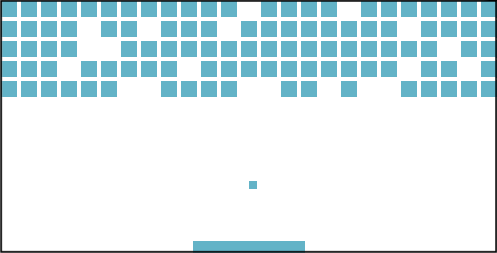
\includegraphics[width=.23\textwidth]{breakout1}\hspace{5pt}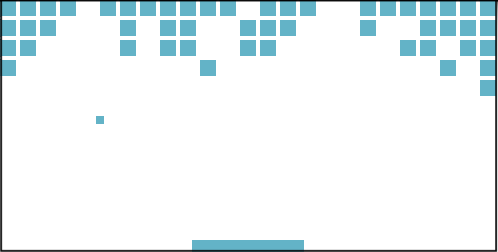
\includegraphics[width=.23\textwidth]{breakout2}
\caption{Breakout game screenshots: the start of a level (left) and after some bricks have been broken (right). The paddle is at the bottom center and the smaller square represents the ball.}
\label{fig:breakout}
\end{figure}

The game's source code was designed to be abstract and decoupled from the hardware (underlying MCU, its peripherals, and the display), enabling portability with minimal modifications. The architecture defines interfaces for core hardware components: the MCU (\autoref{lst:imcu}), digital ports (\autoref{lst:iports}), display, and databus. The display interface is built over a canvas abstraction, which renders to an off-screen buffer. Concrete implementations were developed for the ATmega328P MCU \cite{atmel328p} (\autoref{lst:avr5}) and for an SSD1306 SPI-based display \cite{ssd1306}. There are concrete implementations of the databus interface for both SPI and UART serial communication protocols. At the core of the application, a game class encapsulates the logic and interprets input signals (via UART) to control the paddle’s movement. The architecture of interfaces and types allows easy modification of the SPI display with a corresponding one using I2C protocol, rewiring digital ports, or even replacing the MCU: the same logic runs across different hardware configurations with no changes in the core logic.

We implemented five versions of the game: \emph{rob}, using the prototype language with compiler-driven DI; \emph{vtable}, using C++ OOP, with interfaces implemented as structs with virtual methods, generic programming in strategically chosen places (templates for repeated code), and hard-coded dependencies; \emph{vtabledi}, same as \emph{vtable} but using a compile-time DI framework \cite{boostdi2018} instead of hard-coded dependencies; \emph{concept}, using C++20 concepts instead of virtual dispatch, with hard-coded dependencies; and \emph{conceptdi}, same as \emph{concept} but using compile-time DI. In the following, we discuss some challenges related to software quality attributes, such as cohesion and maintainability for each version. We choose the Boost-ext.di framework \cite{boostdi2018} for implementing compile-time DI in the C++ versions. The framework itself is implemented in a unique header file, without dependencies, can be built without exceptions, and supports the binding of C++ concepts. The complete source code for each game version is available at \blindreview{\url{https://github.com/thborges/sblp2025}}.


\autoref{lst:cppintfsconcept} shows the {\tt digitalport} interface implementation for each C++ breakout game version. For comparison, the implementation for the \emph{rob} version is in \autoref{lst:iports}. C++ does not have interfaces, but they can be implemented as structs (or classes) with virtual methods (lines 2--6). The {\tt =0} indicates a pure virtual function without implementation, making the struct abstract (uninstantiable). Derived classes override these functions and enforce the compiler to use vtables. In contrast, lines 9--14 present the C++20 concept implementation. Distinctly, the concept is only a compile-time constraint that specifies the requirements a type must satisfy to serve as a template parameter. For example, the dependent concrete type {\tt avr5spi}, in lines 17--21, is a template class that requires its dependency ({\tt reset\_port}) to satisfy the {\tt digitalport} concept. Any overhead in size or performance comes from the template usage in the concrete type and not from the concept itself. Note that the {\tt avr5spi} definition does not declare that it implements a databus concept; however, it is necessary as a template parameter in the dependent class. Despite the verbosity of the C++ language, which impacts readability and maintainability, in the virtual struct with the dispensable {\tt virtual} and {\tt =0}, and more pronounced in the concept version,\footnote{The concept is a powerful construct of C++20 that can be used in many other compile-time checks other than the one shown here.} the constructs are equivalent in functionality. In the prototype language, the use of the {\tt interface} keyword (\autoref{lst:iports}) indicates the nature of the construct, dispensing additional symbols.



\lstset{language=c++,morekeywords=[2]{concept,requires,same_as}}
\begin{lstlisting}[float=bp, caption=C++ interface implementation using abstract struct and concepts., label=lst:cppintfsconcept]
// virtual digitalport for vtable versions
struct digitalport {
    virtual void mode(port_mode m) = 0;
    virtual void set(bool v) = 0;
    virtual bool get() = 0;
};

// concept based digitalport
template<typename T>
concept digitalport = requires(T obj) {
    { obj.mode(port_mode{}) } -> same_as<void>;
    { obj.set(bool{}) } -> same_as<void>;
    { obj.get() } -> same_as<bool>;
};

// use of the concept in a concrete type
template<digitalport dp>
class avr5spi {
    dp& reset_port;
    ...
};
\end{lstlisting}




\lstset{language=c++,morekeywords=[3]{bind,to,named}}
\begin{lstlisting}[float=bp, caption=Injectors for each DI-enabled version of breakout game., label=lst:cppbindings]
// injector for the vtabledi version
auto breakout_injector = make_injector(
  bind<mcu>.to<avr5mcu>(),
  bind<buffer8>.to<ssd1306_framebuffer>(),
  bind<display>.to<ssd1306>(),
  bind<databus>.named(nm_uart).to<avr5_uart0>(),
  bind<databus>.named(nm_display).to<avr5_spi>(),
  bind<digitalport>.named(dp_ss).to<avr5mcu_b2>(),
  bind<digitalport>.named(avr5_ss).to<avr5mcu_b2>()
  ... // 5 more bindings for b0, b1, b3 -- b5
};

// injector for the conceptdi version
using spi_t = avr5_spi<avr5mcu_b3, avr5mcu_b4, avr5mcu_b5, avr5mcu_b2>;
using display_t = ssd1306<spi_t, avr5mcu_b1, avr5mcu_b0, avr5mcu_b2, avr5mcu, ssd1306_framebuffer>;

auto breakout_injector = make_injector(
  bind<c_mcu>.to<avr5mcu>(),
  bind<c_databus_uart0>.to<avr5_uart0>(),
  bind<c_buffer8>.to<ssd1306_framebuffer>(),
  bind<c_databus_display>.to<spi_t>(),
  bind<c_display>.to<display_t>(),
  bind<c_digitalport_b2>.to<avr5mcu_b2>(),
  bind<c_avr5_ss>.to<avr5mcu_b2>()
  ... // 5 more bindings for b0, b1, b3 -- b5
};

// injector for the rob version
bind avr5mcu to mcu {
  bind b0 to ssd1306.reset;
  bind b1 to ssd1306.datacmd;
  bind b2 to ssd1306.select;
  bind uart0 to dbus_uart;
  bind spi to dbus_display, ssd1306.dbus;
};
\end{lstlisting}

\autoref{lst:cppbindings} shows the setup of the binding rules for \emph{vtabledi} and \emph{conceptdi}. The injector for \emph{vtabledi} version, lines 2--11, presents the aforementioned use of named bindings ({\tt nm\_uart}, {\tt nm\_display}, {\tt dp\_ss}, and {\tt avr5\_ss}). These names have to be shared between all classes that use them (the main app and the ssd1306 display classes), which reveals as a potential source of name collisions when using libraries provided by distinct vendors or ambiguity if distinctiveness of names is enforced, as exemplified in lines 8 and 9, two names for the same concrete class {\tt avr5mcu\_b2}. These aspects reduce modularity and extensibility.


The concept-based injector for the \emph{conceptdi} version, lines 14--26 of \autoref{lst:cppbindings}, presents a template-heavy configuration that nests templates for the display type (line 15) and the SPI databus (line 14), with additional parameters for three digital ports and a framebuffer. Although the {\tt using} keyword (C++11) allows a split definition, maintaining such code is challenging and heavily depends on understanding the underlying templates (e.g., the order of template parameters). Another problem is the ambiguity caused by the repeated use of the {\tt avr5mcu\_b2} port both in the type definition (lines 14 and 15) and the bindings (lines 23 and 24). A misconfiguration of any of these lines will pass undetected and cause runtime malfunctioning. Furthermore, the compiler error messages often will not aid in diagnosing issues effectively. Thus, we consider it low in maintainability and readability.

Finally, lines 29--35 in \autoref{lst:cppbindings} show the injector for the \emph{rob} version. The use of inner classes allows a concise and centralized expression of binding rules, mapping the relationships between high-level components (e.g., the display to data buses) and low-level MCU resources (e.g., digital ports, UART0, and SPI), which improves readability and enhances modularity. Moreover, inner classes prevent unnecessary exposure of hardware details: for instance, ports {\tt b3}, {\tt b4}, and {\tt b5}, which are fixed for the SPI peripheral in the AVR5 platform, are kept internal and hidden from the top-level configuration. That is impossible in the other DI versions. Thus, we believe that this approach reduces cognitive overhead and the risk of misconfiguration, improving the maintainability and portability of the overall design.

%A summary of quality attributes is presented in \autoref{tab:di_comparison}.



\section{Performance and Size Evaluation} \label{sec:performance}

We evaluated the impact of each game version on the firmware size, instruction count, and runtime performance. The C++ source code was built with {\tt clang++} version 19.1.2 using {\tt -Oz}, {\tt -fno-exceptions}, {\tt -ffunction-sections}, {\tt -fno-rtti}, {\tt -fdata-sections}, and {\tt -lto=thin}. The compiler of the prototype language used the same LLVM 19.1.2 backend and build options. 

The resulting firmware sizes are shown in \autoref{tab:profilebreakout}. The firmware built for \emph{rob} is $4234$ bytes ($41.9\%$) smaller than \emph{vtabledi}, and $3492$ bytes ($37.3\%$) smaller than \emph{conceptdi}. These are the three versions with DI support. The use of the DI framework added $3222$ bytes in the \emph{concept} version and $1406$ bytes in \emph{vtable}, a significant amount of memory for an MCU. \emph{Rob} size is also smaller compared to \emph{vtable} ($32.5\%$) and \emph{concept} ($4.4$\%). Note the effectiveness of the concepts feature regarding the binary size. The main cause for the larger size of \emph{vtable} is the use of vtables itself, which increases call overhead, producing significant stack manipulation and reducing the efficiency of some compiler optimization passes (inlining, constant propagation, DCE, IPO). Both \emph{concept} and \emph{rob} firmware do not produce vtable structures, and their size difference stems from the \emph{concept's} reliance on generic programming and minor variations in compiler inlining and optimizations.


\begin{table}[bp]
\caption{Size (in bytes) and performance measured as fps of each breakout game implementation.}\vspace{-8pt}
\label{tab:profilebreakout}
\begin{tabular}{lrrrrrr}
\toprule
\bf version & \bf size & Δ\% & \bf fps & Δ\% \\
\midrule
\emph{vtabledi}   & 10108 & --     & 2925 & +4.4     \\
\emph{vtable}     & 8702  & -13.9  & 2801 & --   \\
\emph{conceptdi}  & 9366  & -7.3   & 3948 & +41.0  \\
\emph{concept}    & 6144  & -39.2  & 3972 & +41.8  \\
\emph{rob}        & 5874  & -41.9  & 4855 & +73.3  \\
\bottomrule
\end{tabular}
\end{table}

%    Five implementations of breakout. Results:
%                             time
%    version          size     hw   sim
%    rob              5874   13.5   4.4
%    cppconcept       6144   16.5   5.4
%    cppconceptdi     9366   16.6   5.5
%    cppvtable        8702   23.4   7.6
%    cppvtabledi     10108   22.4   7.3

To measure performance, we deactivated the game-over condition and allowed the game to continue when the ball hit the bottom edge as if the paddle was there. We also let the game run at full speed, without time constraints imposed at normal execution. In this approach, we run all levels and measure the time to complete the game ($t$), count frame updates ($u$), and compute frames per second (fps) as fps=$u/t$. We captured the start and the end of the game execution through the {\tt uart0} port. 

%, running at 115200 bauds (sufficient to prevent I/O-induced firmware blocking).

%and in a custom Simavr based simulator with support to the SPI display.\footnote{Available at \url{https://github.com/buserror/simavr}; changes in the fork \blindreview{\url{https://github.com/thborges/simavr}}.}

The results are shown in \autoref{tab:profilebreakout}, under the fps column. The \emph{rob} implementation was $73.3\%$ faster than \emph{vtable}; \emph{vtabledi} runs $4.4\%$ more frames per second than \emph{vtable}, followed by \emph{conceptdi} ($41\%$) and \emph{concept} ($41.8\%$). The reason for the difference in performance is the reduction in the total number of instructions (simplification of critical paths) and the use of simpler, faster instructions. The rob version reduced costly operations such as indirect calls ({\tt icall}, 3 clock cycles) and performed significantly fewer memory and stack operations, such as {\tt movw}, {\tt ldd}, {\tt ld}, {\tt push}, and {\tt pop}. The vtable version, by contrast, introduces extra overhead through indirect calls and increased memory manipulation, while the concept version, though avoiding {\tt icall}, still exhibits more stack manipulation than rob. In summary, the compiler-driven dependency injection exposed better inlining and optimization opportunities that remain hidden in the C++ code.


\begin{table}[bp]
\caption{Instruction count comparison for the breakout game firmware. The hidden rows have $-20 \le \Delta \le 9$.}\vspace{-8pt}
%The reduction in rob of $1,537$ ($36.4\%$) instructions compared to vtables, and $518$ ($16.2\%$) instructions compared to concepts, are primarily due to significant decreases in memory and stack related operations ({\tt movw}, {\tt mov}, {\tt ldd}, {\tt ld}, {\tt push}, {\tt pop}) as well as the elimination of indirect calls ({\tt icall}).
\label{tb:mnemonicscount}
\begin{tabular}{lrrrrr}
\toprule
& & \multicolumn{4}{c}{\bf C++} \\
\cmidrule{3-6}
\bf Instr. & \bf rob & \bf vtables & Δ & \bf concepts & Δ \\
\midrule
movw & 173 & 594 & -421 & 309 & -136 \\
ldd & 73 & 359 & -286 & 114 & -41 \\
ld & 8 & 137 & -129 & 35 & -27 \\
pop & 87 & 174 & -87 & 132 & -45 \\
push & 87 & 174 & -87 & 132 & -45 \\
icall & 0 & 63 & -63 & 0 & 0 \\
lds & 13 & 68 & -55 & 46 & -33 \\
ret & 65 & 118 & -53 & 72 & -7 \\
mov & 141 & 190 & -49 & 161 & -20 \\
add & 86 & 126 & -40 & 109 & -23 \\
sbci & 71 & 107 & -36 & 87 & -16 \\
adc & 109 & 140 & -31 & 123 & -14 \\
subi & 60 & 89 & -29 & 69 & -9 \\
eor & 102 & 126 & -24 & 115 & -13 \\
or & 11 & 33 & -22 & 23 & -12 \\
sbc & 25 & 46 & -21 & 45 & -20 \\
\multicolumn{6}{c}{...} \\
in & 66 & 57 & 9 & 28 & 38 \\
out & 77 & 66 & 11 & 39 & 38 \\
dec & 29 & 14 & 15 & 14 & 15 \\
ldi & 213 & 195 & 18 & 146 & 67 \\
cpi & 76 & 55 & 21 & 48 & 28 \\
sts & 25 & 2 & 23 & 2 & 23 \\
adiw & 50 & 22 & 28 & 18 & 32 \\
std & 236 & 129 & 107 & 102 & 134 \\
\midrule
 & 2762 & 4060 & -1298 & 2878 & -116 \\
\bottomrule
\end{tabular}
\end{table}

We further investigated the reason behind this result by disassembling the firmware ELF binaries with the utility command {\tt avr-objdump -D} and a custom Python script to count how many times each instruction mnemonic appeared in the disassembled code. The results are shown in \autoref{tb:mnemonicscount}. \emph{Rob} firmware has $1298$ fewer instructions than \emph{vtable}, representing a $32\%$ decrease in instruction count. Compared to \emph{concept}, \emph{rob} also presented $116$ fewer instructions ($4\%$). The most reduced instructions compared to \emph{vtable} are memory-related operations ({\tt movw}: $-421$, {\tt ldd}: $-286$, {\tt ld}: $-129$) and call stack manipulations ({\tt push}: $-87$, {\tt pop}: $-87$), reflecting the elimination of vtable lookups and reduced call overhead. These are also the most reduced instructions when compared with \emph{concept}. Notably, {\tt icall} instructions were eliminated (\emph{vtable}: $63$, \emph{concept} and \emph{rob}: 0), demonstrating the effectiveness in eliminating runtime indirection by the use of concepts and compiler-driven dependency injection. 

The increase of \texttt{std} ($+134$) and \texttt{ldi} ($+67$) in \textit{rob} occurs during the initialization of variables and bindings, a one-time operation, whereas the reductions in \texttt{ldd} ($-286$) and \texttt{push} ($-87$) benefit the game's main loop. This trade-off is advantageous, as the continuous frame rendering amortizes the initialization overhead.

%Although some instructions, such as {\tt std} ($+134$) and {\tt ldi} ($+67$), increased in rob, they reflect specific instance bindings at initialization adopted by the language and were compensated by consequent optimizations. 


%Although the firmware size for concept does not show a significant difference, the type of instructions used 


\section{Conclusion and Future Work} \label{sec:conclusion}

In this paper, we addressed the challenges of developing maintainable and optimized software for resource-constrained embedded systems. Traditional OOP approaches often introduce unwanted runtime overheads due to their low-level implementation of polymorphism (vtables with dynamic dispatch). While alternative language features, such as generic programming (templates) and C++20 concepts, do eliminate dynamic dispatch in favor of static dispatch, they also introduce challenges regarding readability and maintainability due to their verbosity and complex metaprogramming constructs. 

To overcome these limitations, we proposed a novel compiler-driven dependency injection approach deeply integrated into a prototype language. The design shifts the responsibility of dependency resolution from runtime (or library-based metaprogramming at compile-time) to the language frontend and compiler intermediate representation. The strategic binding points and a concise bind syntax allowed the compiler to perform static dependency injection by replacing interface types with concrete implementations in the Abstract Syntax Tree (AST).

Our comprehensive case study, a breakout game implemented in five distinct versions (including C++ OOP, C++20 Concepts, and boost-ext.di frameworks), provides empirical evidence of the language syntax adherence to the targeted application domain. The \emph{rob} implementation consistently shows smaller firmware sizes (e.g., 41.9\% smaller than \emph{vtabledi}) and higher runtime performance (e.g., 73.3\% faster than \emph{vtable}). A disassembly analysis revealed the underlying reasons: compiler-driven DI eliminated costly runtime indirections, such as vtable lookups and icall instructions, and exposed opportunities for optimization passes, reducing memory and stack operations. 

Beyond the quantitative gains, language features such as inner classes and the bind statement improve maintainability, enhance early error detection for missing or incorrect dependencies, and reduce cognitive overhead by providing a coherent, language-native mechanism for managing component relationships.

Looking forward, our work opens some avenues for future research. We plan to explore the expansion of the language features to support more complex dependency patterns and how to incorporate other binding scopes, such as transient, feature-specific, or thread-local dependencies. Furthermore, we aim to evaluate our compiler-driven paradigm on a broader range of embedded software to further validate its benefits across diverse hardware platforms.

\bibliographystyle{ACM-Reference-Format}
\bibliography{sblp2025}

\end{document}

